\chapter{Other results}
\label{cpt:other}
\section{Introduction}
Due to the complexity of financial market and the interconnectedness and interdependencies of industrial sectors in the economy, the price returns of each coupling stocks might have certain underlying economic link. Such behaviours can hardly be explained by traditional financial models and theories. This chapter attempts to combine machine learning techniques, individual stock features, and empirical data of Economic Input-Output (EIO) from Bureau of Economic Analysis (BEA) in the US to predict Granger causality of coupling US stocks. Limited Granger causalities are calculated as a small sample set compared to the target date set. Therefore a directed complex network is expected to be constructed. The generated directed stock network is planned to be analysed about its topological properties, stability and effects on individual stocks and industries. Suggestions towards financial market investment are expected to be provided based on the results in this study.

Financial data of listed companies and fundamental economical data are both available in each stock market and government websites. Efforts have been taken upon the researches such as the work of Patel et al. \cite{patel2015predicting}, which applied machine learning techniques to predict stock price movement, but most of them use correlations between stock price or return series, such measures are unable to provide direction information for building a directed graph of stock market. Granger causality test is one suitable measure but the computation is overwhelmingly complex so that no researchers have ever implemented this.

This chapter has probed into the feasibility of applying machine learning techniques helping to predict Granger causality based on samples of Granger causalities that have been manually calculated. Here the word “predict” means estimation of some property that is not directly observed, rather than its common meaning of inferring something about the future. Unfortunately, over 3,000 listed companies yielding couples many orders of magnitude larger than the amount of sample data for human-beings can ever calculate. The scarcity of training data on these outcomes makes the application of machine learning techniques challenging.

This project overcome this challenge through a multi-step “transfer learning” approach \cite{pan2010survey}, whereby a noisy but easily obtained proxy for sectoral association, the correlations of stock pairs, and fundamental indicators of listed companies are used to train a deep learning model. The model is then used to estimate Granger causalities based on very limited samples through a transferring process.

\subsection{Motivation} % DONE
Conducting Granger causality test between the price return series of all stock pairs is straightforward while not feasible due to the heavy-precondition for Granger causality test in time series analysis and the high time-complexity in computer programme, as this is an NP-hard problem. Hence, predicting Granger causality of the price return series of stock pairs using a training sample which contains manually calculated Granger causalities. However, compared to the large order of magnitude of total stock pairs, the realistic number of manually calculated Granger causalities are too less to be regarded as training samples. Enlightened by the recent work of Jean et al. (2016) which implements transfer learning and noisy proxy information performed unexpectedly well at predicting poverties, demonstrating that machine learning techniques are powerful to be applied in a setting with limited training data \cite{jean2016combining}, therefore an exploration towards the directed network of stock market is motivated in this thesis, combines machine learning techniques, transfer learning, individual stock features, and empirical data of Economic Input-Output (EIO) from Bureau of Economic Analysis (BEA) in the US to predict Granger causalities of rest coupling US stocks. Therefore, the directed stock network is able to be constructed by considering predicted Granger causalities as the indicators of directions of edges.

\subsection{Objectives} % deliverables list
The goal of the attempt in this chapter is to predict and reveal the Granger causality of price return series with machine learning techniques and utilise them into the construction and topological analysis of the directed stock network as so far no previous work has ever been attempted to construct a directed network of stock markets. While in hindsight this is not a successful attempt, conclusion will be drew according to the results of prediction.

\section{Methodology}

\begin{figure}
	\begin{center}
		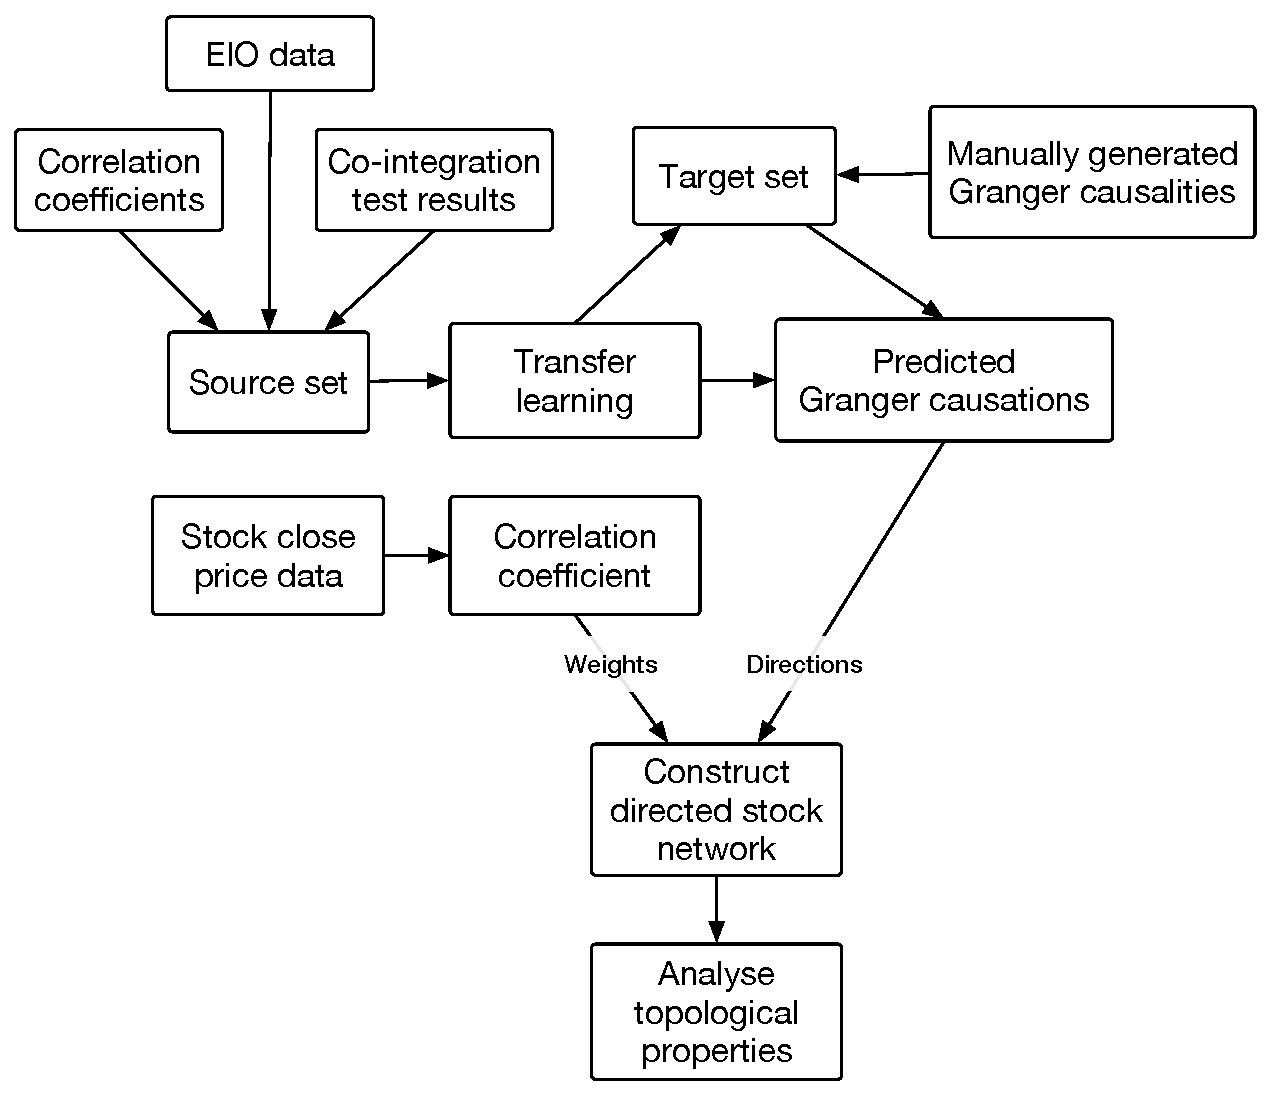
\includegraphics[width=11cm]{methodology_diagram_dnn}
	\end{center}
	\caption{The methodology diagram of machine learning pathway}
	\label{fig:methodology_diagram_dnn}
\end{figure}

\subsection{Technical challenges in the pre-processing for network construction}
A preliminary correlation matrix is generated for the co-integration test of two price return time series. Bivariate Granger causality test is heavy on the precondition of time series analysis and its time-complexity in computer programme is polynomial, as the amount of all coupling stock pair is $n(n-1)/2$, while $n$ is the number of stocks. There are over 3,000 companies listing in NASDAQ, hence there should be millions of times for Granger causality tests and pre-process time series analyses to run in the computer programmes in order to construct the directed stock network.

However, in this chapter, machine learning techniques are applied to predict the precedence relations, i.e., predicted Granger causalities of every possible US stock pairs, based on a limited amount of actual Granger causalities calculated as training set. In addition to the fundamental indicators such as market capitalisation, P/B ratio, P/E ratio, etc., public empirical data of EIO are also implemented into the entire machine learning prediction process. Stocks are divided into industrial groups according to the summary level defined in the BEA. Transfer learning technique is applied as well and will be introduced in section \ref{sbs:transfer}. In addition, learning performances of each models are compared based on their predicting performances according to the ROC analysis.

\subsection{Granger causality test}
Granger causality test \cite{granger1969investigating} provides an asymmetrical measure for testing precedence relationship between two time series. The leitmotiv inside is that a time series can be described and analysed through a time-delayed auto-regressive model. Granger causality test tests whether the difference of a prediction to the time series from another time series through a multi-variate auto-regressive model is able to improve the prediction of the current behaviour of the time series, as the following forms illustrates:

\begin{eqnarray}
&&	x_t=\sum_{i=1}^{\infty}a_ix_{t-i}+c+\varepsilon_{t}\\
&&x_t=\sum_{i=1}^{\infty}a_ix_{t-i}+\sum_{j=1}^{\infty}b_jy_{t-j}+c'+\varepsilon_{t}'
\end{eqnarray}

Calculate the f-statistic using the following equation, the Granger causality is not significant if f-statistic is greater than the f-value:
\begin{eqnarray}
&&	F=\frac{(ESS_R-ESS_{UR})/q}{ESS_{UR}/(n-k)}
\end{eqnarray}

\subsection{Transfer learning and ANN model}
\label{sbs:transfer}
Conventional machine learning normally has two basic assumptions: (1) the training sample and the test sample are both independent and identically distributed; (2) there must be enough available training samples. However, as aforementioned reasons in this chapter, the application of machine learning in stock market to predict Granger causalities is hard to satisfy the assumptions.

Transfer learning with existing knowledge to solve only one small target area labelled sample data even without data of learning problems, fundamentally relaxes the basic assumptions of conventional machine learning. Transfer learning can migrate the models which are applicable to big data sets to small data sets, identifies the commonality of different problems, and then transfer the generalised model on customised data sets to achieve customised transfer.



The ANN model that this thesis has 2 layers and there are 10 nodes in each layers.  The activation function is rectified linear unit (ReLU) \cite{hahnloser2000digital}, as the below expression shows:

\begin{eqnarray}
f\left(x\right)=x^+=max\left(0,x\right)
\end{eqnarray}

During the training process, Adagrad optimiser \cite{duchi2011adaptive} with the learning rate of 0.01 are used.

Since we have only several hundred data points for consumption or assets in each country to be used as labelled training examples, we cannot directly train a large CNN model to estimate these outcomes from satellite images — we simply do not have enough data. Additionally, the task of estimating economic well-being from satellite imagery is nontrivial for human non-experts, precluding the generation of additional labelled training data through crowd-sourcing services such as Amazon Mechanical Turk.

To combat the data scarcity problem, we use a transfer learning method and train a fully-convolutional CNN model on the data-rich nighttime light estimation task. By solving this related proxy task, the model learns how to extract features that are also useful for the poverty estimation task. In previous work (15), we found that a multi-step approach outperforms simpler transfer learning methods that use imagery and nightlight information. For example, a simpler alternative would be to use an off-the-shelf CNN trained on ImageNet to extract image features that could then be used in conjunction with nightlights to predict poverty indicators


% theoretical and practical

\section{Results}
In terms of future work, stock complex networks during a longer range of years can be generated and compared in together, the periods correspond to bull, bear, and stable market can be recognised and analysed separately and accordingly. New methods for determining the directions of edges to generate directed complex networks are expected to be proposed.

\begin{figure} % P-P SW
	\centering
	\subfloat[Accuracy]{
		\label{subfig:accuracy}
		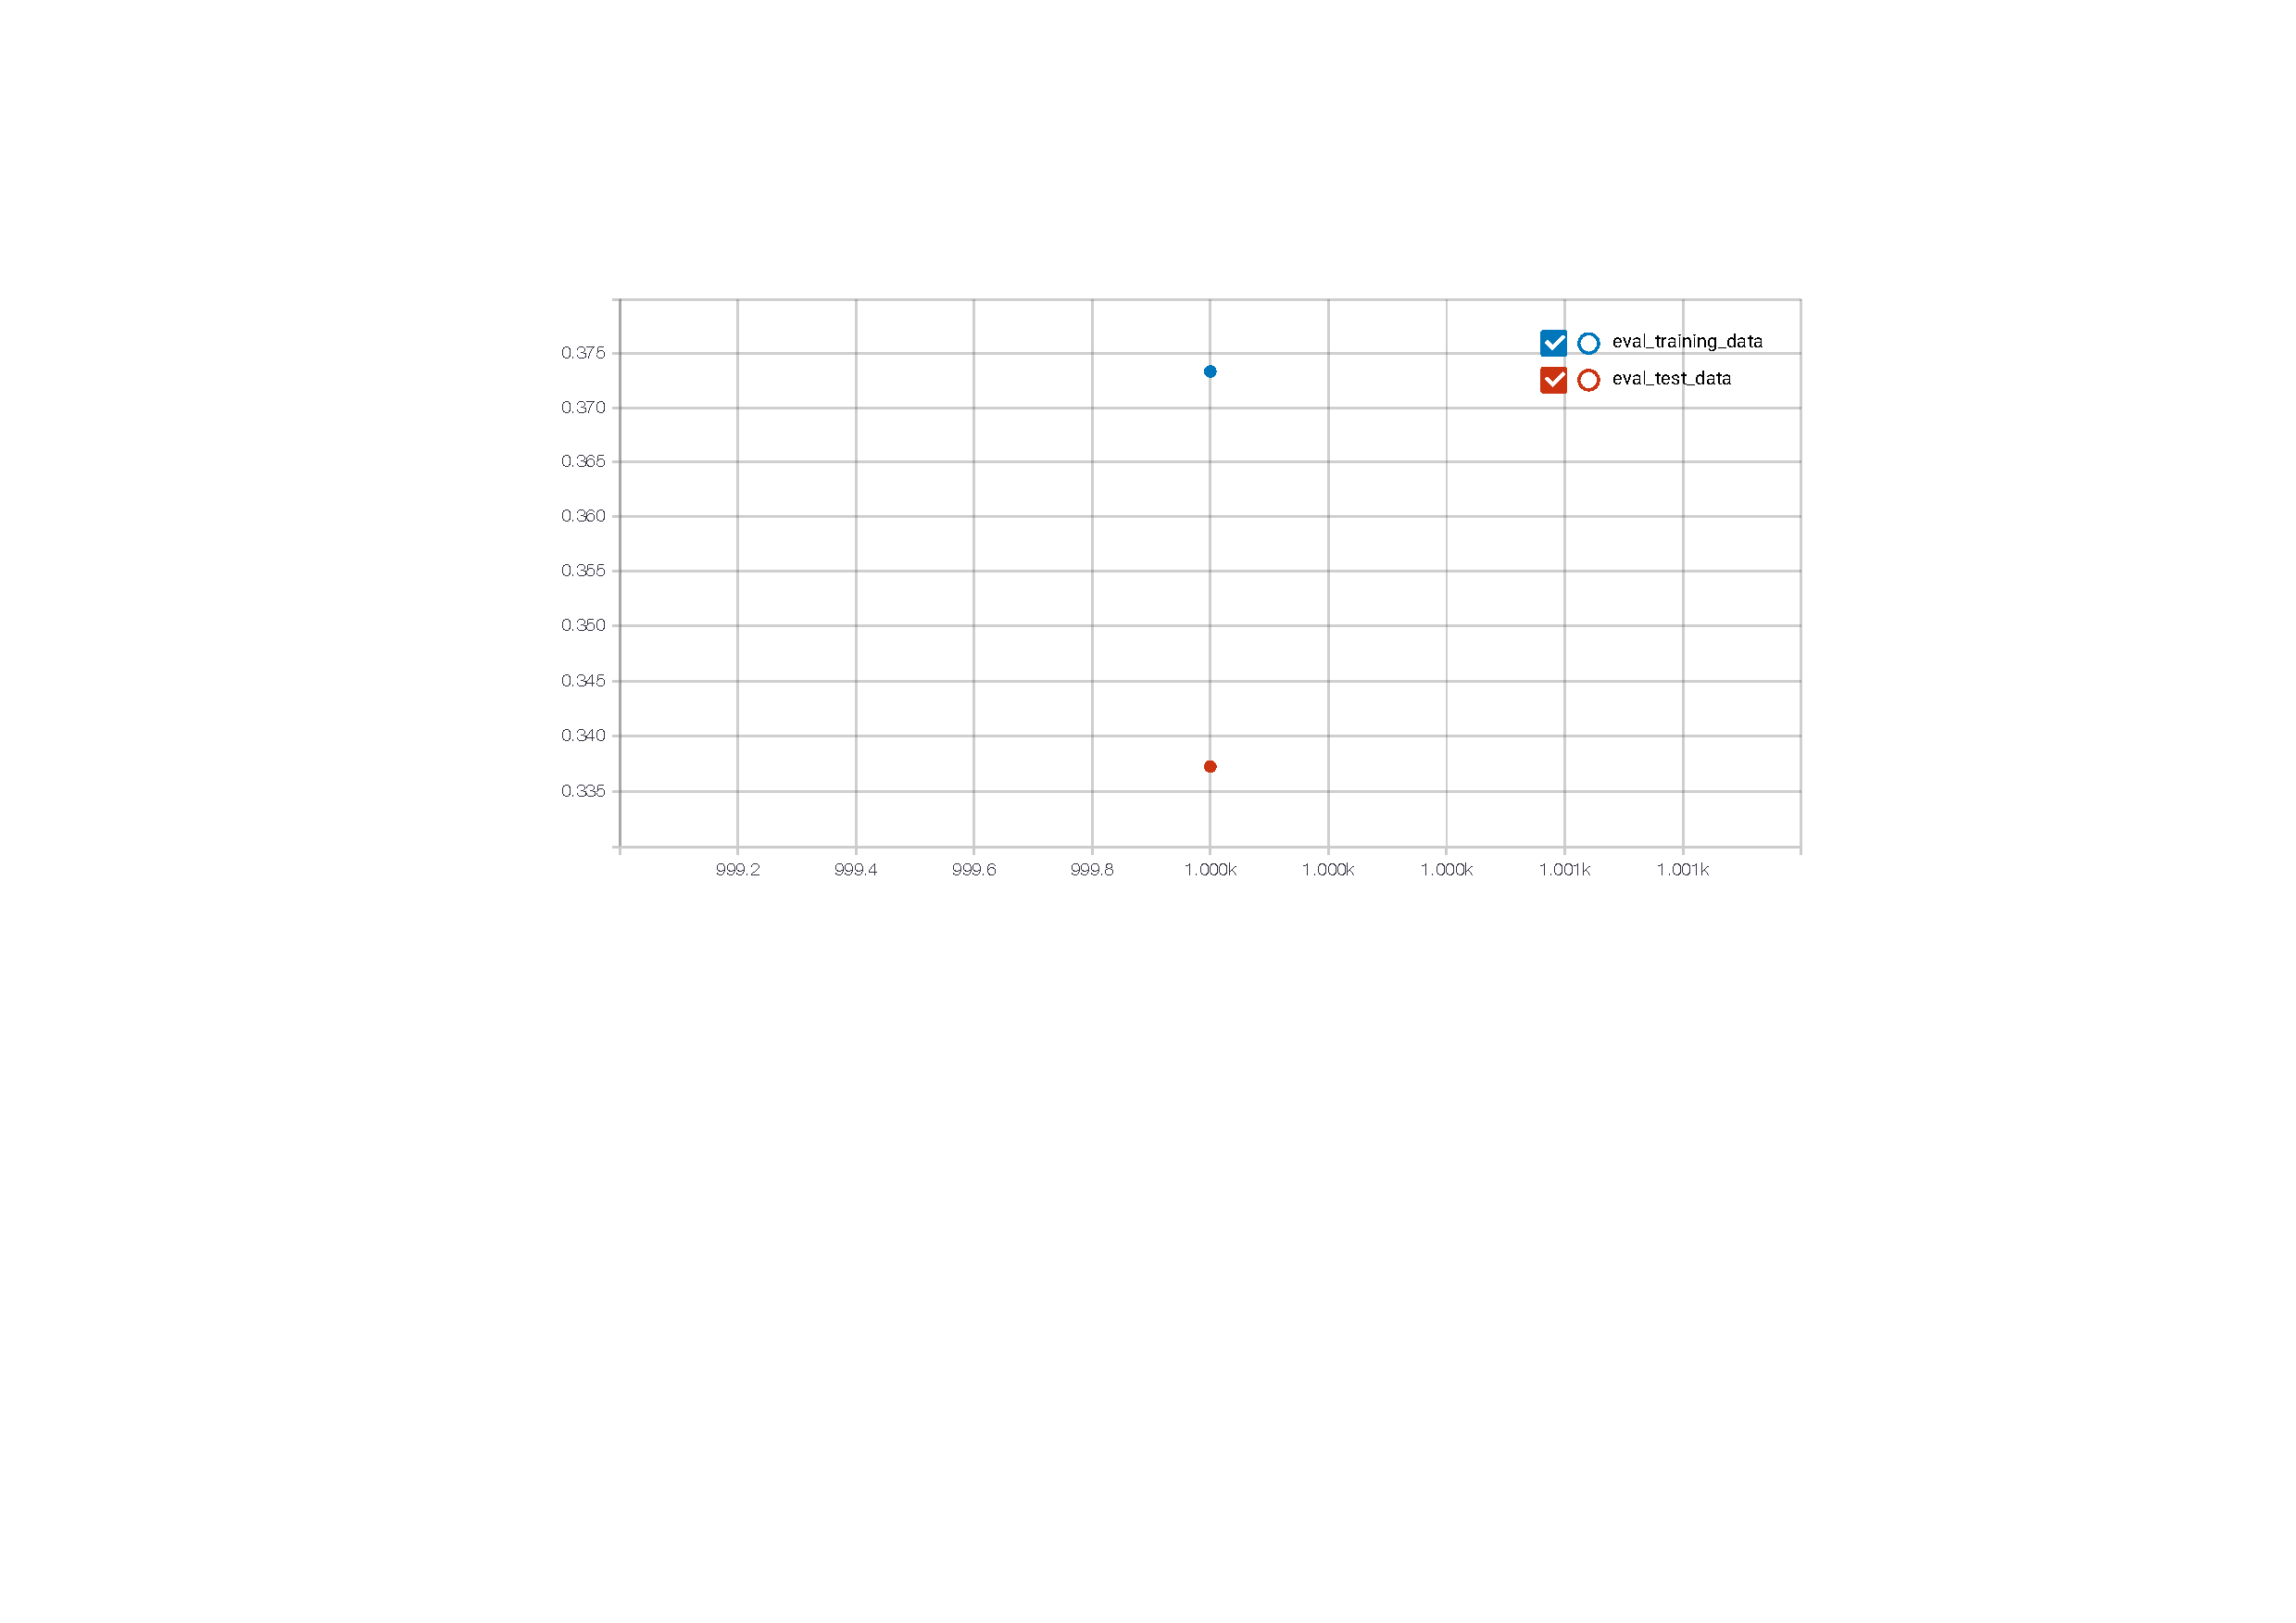
\includegraphics[width=13cm]{accuracy} }
	
	\subfloat[Average Loss]{
		\label{subfig:average_loss}
		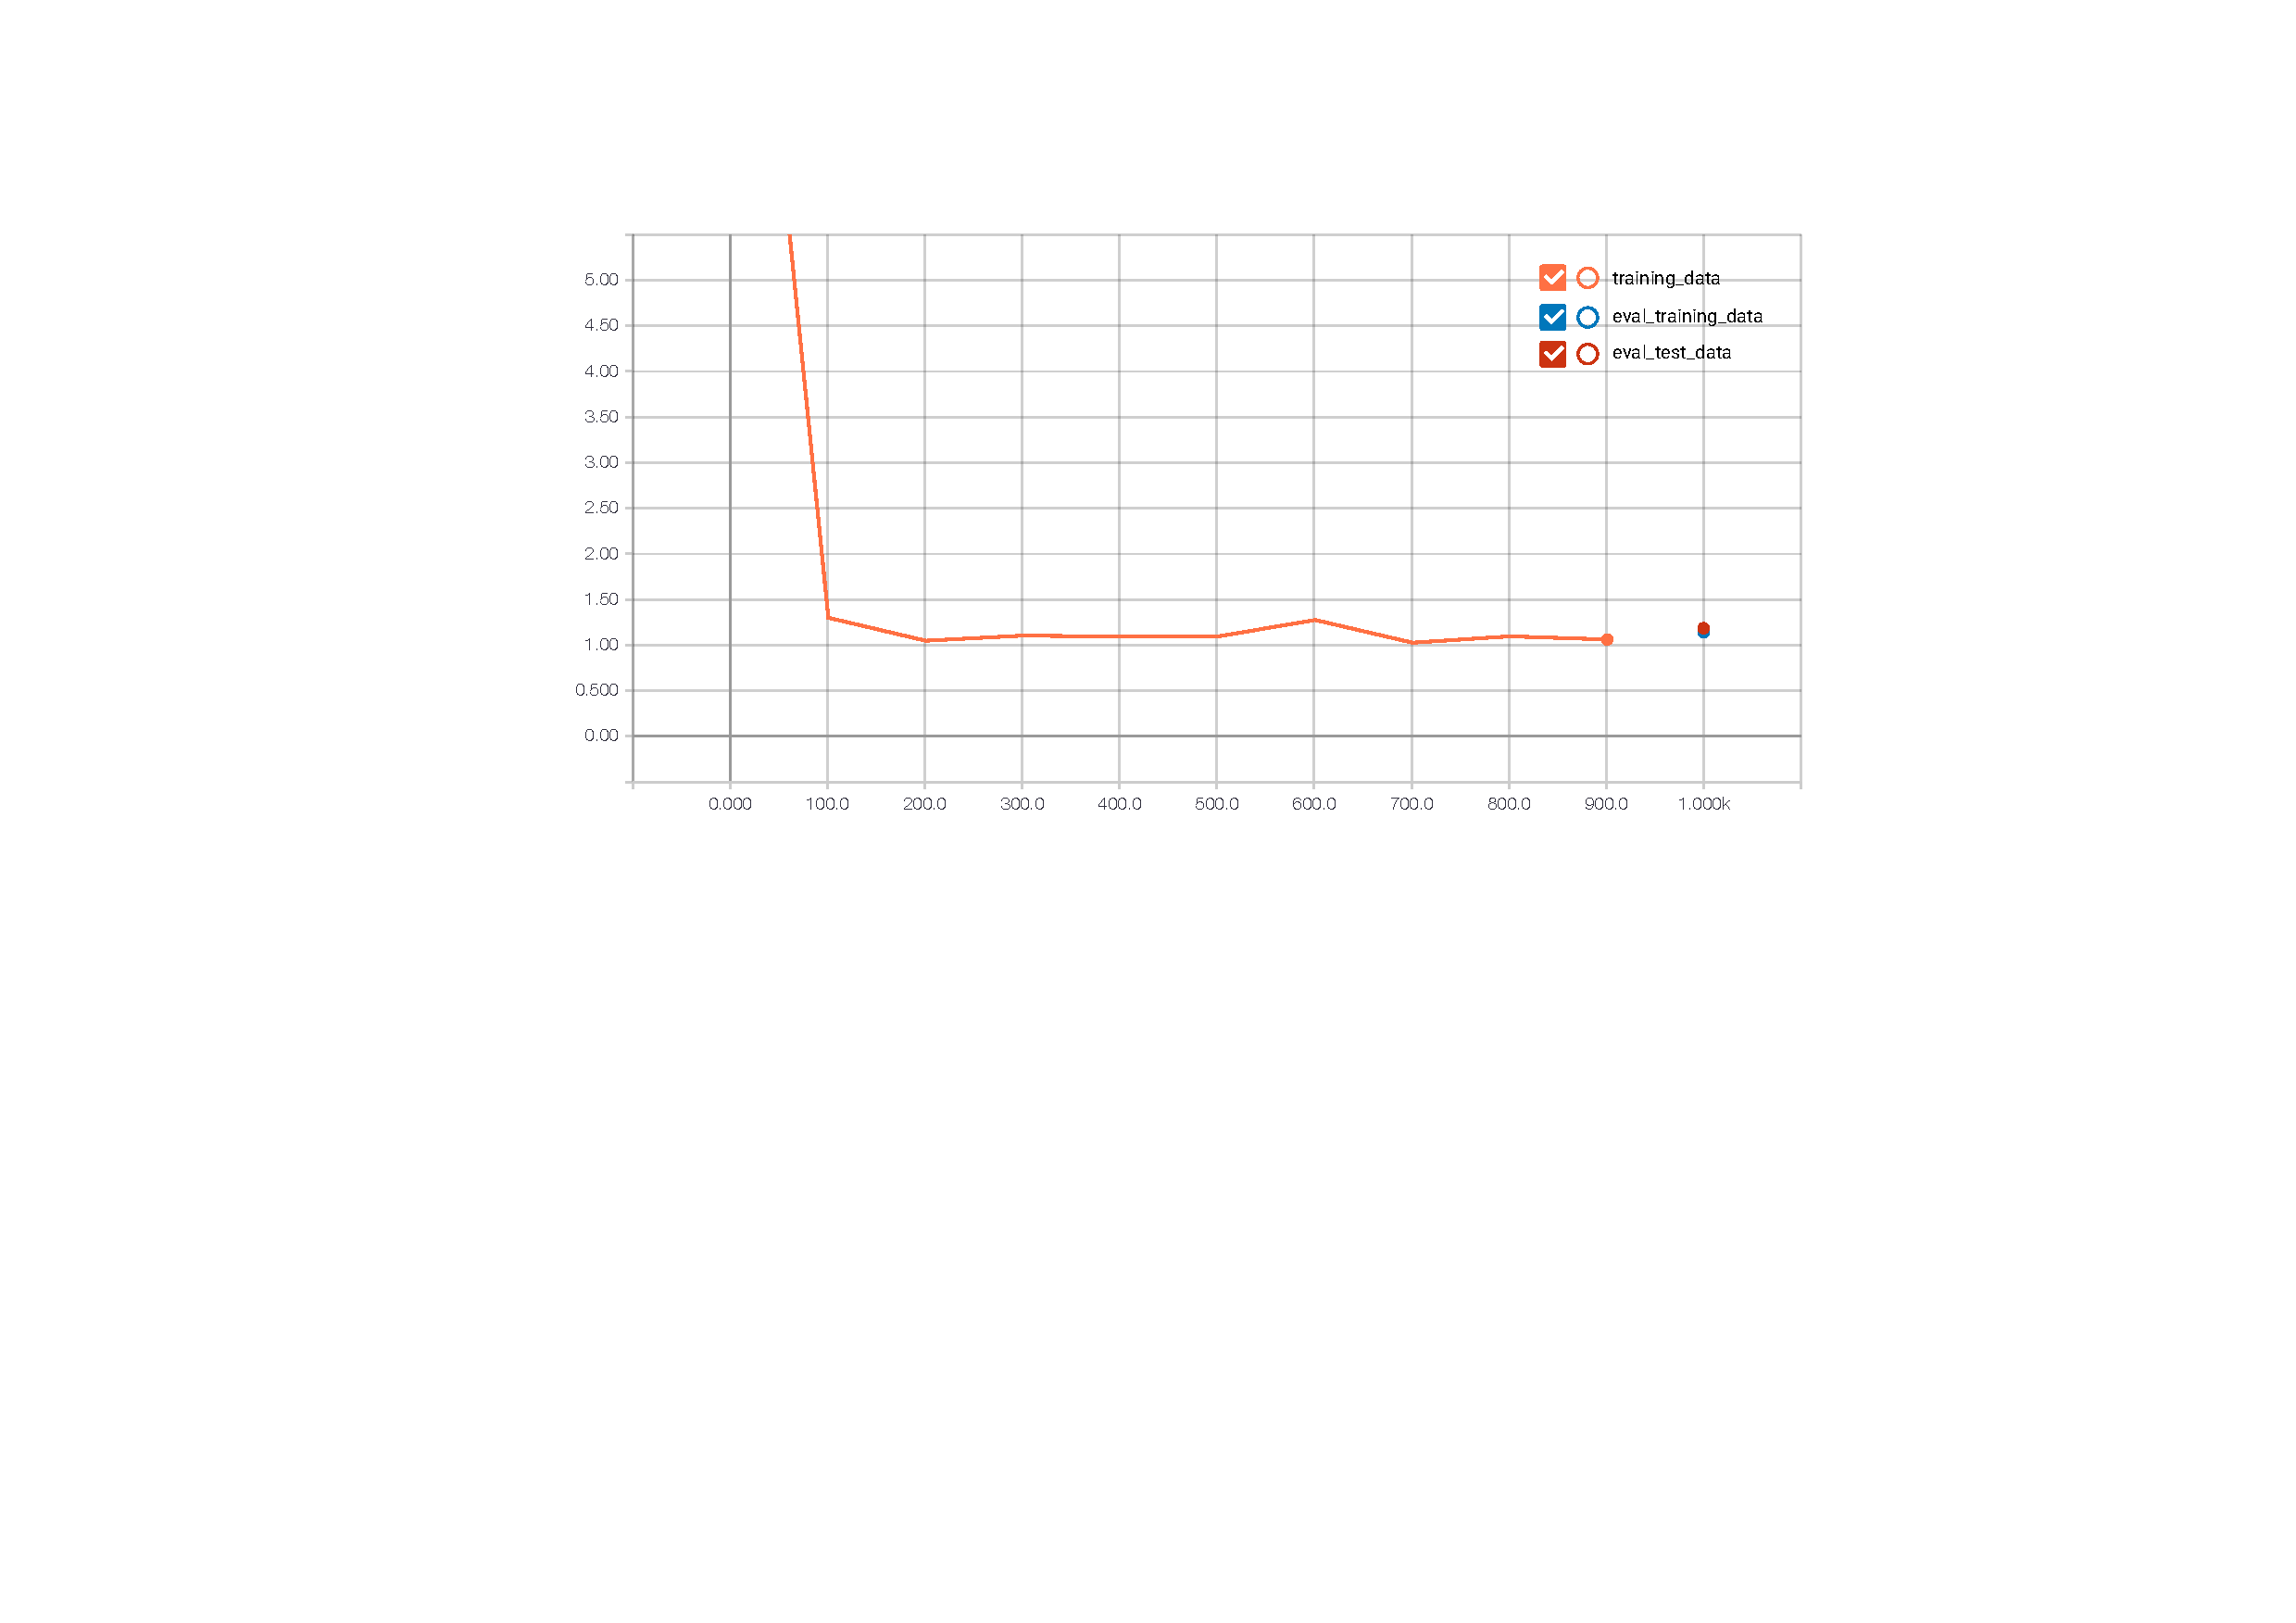
\includegraphics[width=13cm]{average_loss} }
	
	\caption{Performance of prediction. Graphs are generated by \textit{TensorBoard} \cite{tensorflow2015-whitepaper}.}
	\label{fig:prediction}
\end{figure}

\section{Conclusion}
The 

%所以接下来无法进行后续研究
